\documentclass{article}
\usepackage[utf8]{inputenc}
\usepackage{amsfonts}
\usepackage{amsthm} % theorems structure
\usepackage{enumerate}
\usepackage{hyperref} % links
\usepackage{tikz} % diagrams
\usepackage{pgf-umlsd} % diagrams
\usepackage{amsmath} % arrows

\theoremstyle{definition}
\newtheorem{example}{Example}[section]

\title{Sigma protocol and OR proofs - notes}
\author{arnaucube}
\date{March 2022}

\begin{document}

\maketitle

\begin{abstract}
	This document contains the notes taken during the \emph{Cryptography Seminars} given by \href{https://github.com/rbkhmrcr}{Rebekah Mercer}.
\end{abstract}

\tableofcontents

\section{Sigma protocol}

\subsection{The protocol}
Let $q$ be a prime, $q$ a prime divisor in $p-1$, and $g$ and element of order $q$ in $\mathbb{Z}_p^a$. Then we have $G = \langle g \rangle$.
\\
We assume that computationally for a given $A$ it's hard to find $a \in \mathbb{F}$ such that $A = g^a$.
\\
Alice wants to prove that knows the \emph{witness} $w \in \mathbb{F}$, such that the \emph{statement} $X = g^w$, without revealing $w$.

\begin{enumerate}[1.]
	\item Alice generates a random $a \xleftarrow{r} \mathbb{F}$, and computes $A=g^a$. And sends $A$ to Bob.
	\item Bob generates a challenge $c \xleftarrow{r} \mathbb{F}$, and sends it to Alice.
	\item Alice computes $z=a + c \cdot w$, and sends it to Bob.
	\item Bob verifies it by checking that $g^z == X^c \cdot A$.
\end{enumerate}

We can unfold Bob's verification and see that:
$$g^z == X^c \cdot A$$
$$g^{a+cw} == g^{wc} g^a$$
$$g^{a+cw} == g^{wc+a}$$

\begin{center}
\begin{sequencediagram}
    \newinst[1]{a}{Alice}
    \newinst[3]{b}{Bob}
    \mess[0]{a}{$A$}{b}
    \mess[2]{b}{$c$}{a}
    \mess[2]{a}{$z$}{b}
    \mess[0]{b}{$ok$}{a}
\end{sequencediagram}
\end{center}

Properties:
\begin{enumerate}[i.]
	\item \emph{correctness/completness}: if Alice know the witness for the statement, then they can create a valid proof.
	\item \emph{soundness}: if someone does not have knowledge of the witness, can not form a valid proof (verifier will always reject).
	\item \emph{zero knowledge}: nobody gains knowledge of anything new with the proof. prior knowledge + proof = prior knowledge
\end{enumerate}

\subsection{Non interactive protocol}
With the \emph{Fiat-Shamir Heuristic}, we model a hash function as a random oracle, thus we can replace Bob's role by a hash function in order to obtain the challenge $c \in \mathbb{F}$.
\\
So, we replace the step 2 from the described protocol by $c = H(X || A)$ (where $H$ is a known hash function).

\subsection{What could go wrong (Simulator)}
If the verifier (Bob) sends $c \in \mathbb{F}$, prior to the prover committed to $A$, the prover could create a proof about a public key which they don't know $w$.
\begin{enumerate}[1.]
	\item Bob sends $c \xleftarrow{r} \mathbb{F}$ to Alice
	\item Alice generates $z \xleftarrow{r} \mathbb{F}$
	\item Alice then computes $A = g^z X^{-c}$, and sends $z, A$ to Bob
	\item Bob would check that $g^z == X^c A$ and it would pass the verification, as $g^z== X^c \cdot A \Rightarrow g^z==X^c \cdot g^z X^{-c} \Rightarrow g^z == g^z$.
\end{enumerate}

As we've seen, it's really important the order of the steps, so Alice must commit to $A$ before knowing $c$.\\
This 'fake' proof generation is often called the \emph{simulator} and used for further constructions.

\section{OR proof}

\emph{OR proofs} allows the prover to prove that they know the witness $w$ of one of the two known \emph{public keys} $X_0, X_1 \in \mathbb{F}$, without revealing which one. It uses the construction seen in the \emph{sigma protocols} together with the idea of the \emph{simulator}.

A similar construction is used for $n$ statements in the \emph{ring signatures} scheme (used for example in \emph{Monero}). In our case, we will work with $n=2$.

\subsection{The protocol}
\subsubsection{Simulator}
We can assume that the simulator is a box that for given the inputs $(g, X)$, it will output $(A_s, c_s, z_s)$, such that verification succeeds ($g^{z_s}==X^{c_s} \cdot A_s$).

\begin{center}
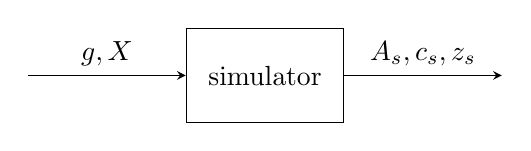
\begin{tikzpicture}
\node [draw,
    minimum width=2cm,
    minimum height=1.2cm,
    right=1cm
    ]  (simulator) {simulator};
\draw[-stealth] ++(-1,0) -- (simulator.west)
    node[midway,above]{$g, X$};
\draw[-stealth] (simulator.east) -- ++(+2,0)
    node[midway,above]{$A_s, c_s, z_s$};
\end{tikzpicture}
\end{center}

Internally, the simulator computes
$$z_s \xleftarrow{r} \mathbb{F},~c_s \xleftarrow{r} \mathbb{F},~A_s = g^{z_s} \cdot X^{c_s}$$

\subsection{Flow}
For two known \emph{public keys} $X_0, X_1 \in G$, Alice knows $w_b \in \mathbb{F}$, for $b \in \{0, 1\}$, such that $g^{w_b} = X_0$ or $g^{w_b} = X_1$. As we don't know if Alice controls $0$ or $1$, from now on, we will use $b$ and $1-b$.
\\
So, Alice knows $w_b \in \mathbb{F}$ such that $X_b = g^{w_b}$, and does not know $w_{1-b}$ for $X_{1-b}=g^{w_{1-b}}$.

\begin{enumerate}
    \item First of all, as in the \emph{Sigma protocol}, Alice generates a random \emph{commitment} $a_b \xleftarrow{r} \mathbb{F}$, and computes $A_b = g^{a_b}$.
    \item Then, Alice will run the \emph{simulator} for $1-b$.
	\begin{list}{}
	    \item Sets a random $c_{1-b} \xleftarrow{r} \mathbb{F}$, and runs the simulator with inputs\\$(c_{1-b}, X_{1-b})$, and outputs $(A_{1-b}, c_{1-b}, z_{1-b})$.
	    \item Remember that internally the \emph{simulator} will set random\\
		$z_{1-b}, c_{1-b} \xleftarrow{r} \mathbb{F}$, and compute an $A_{1-b}$ such that\\
		$A_{1-b} = g^{z_{1-b}} \cdot X_{1-b}^{c_{1-b}}$.
	\end{list}
	\item Now, Alice sends $A_b, A_{1-b}$ to Bob
	\item And Bob sends back the \emph{challenge} $s \xleftarrow{r} \mathbb{F}$.
	\item Alice then splits the challenge $s$ into $c_b, c_{1-b}$, by $s = c_{1-b} \oplus c_b$. So Alice can compute $c_b = s \oplus c_{1-b}$.
	\item Then Alice computes $z_b = a_b \cdot w_b + c_b$. And sends to Bob $(c_b, c_{1-b}, z_b, z_{1-b})$.
	\item Bob can perform the verification by checking that:
	\begin{enumerate}[i.]
	    \item $s == c_b \oplus c_{1-b}$
	    \item $g_{z_{1-b}} == A_{1-b} \cdot X_{1-b}^{-c_{1-b}}$
	    \item $g_{z_b} == A_b \cdot X_b^{-c_b}$
	\end{enumerate}
\end{enumerate}



\begin{center}
\begin{sequencediagram}
    \newinst[1]{a}{Alice}
    \newinst[3]{b}{Bob}
    \mess[1]{a}{$A_b, A_{1-b}$}{b}
    \mess[1]{b}{$s$}{a}
    \mess[1]{a}{$c_b, c_{1-b}, z_b, z_{1-b}$}{b}
\end{sequencediagram}
\end{center}

\section{Resources}
\begin{enumerate}
    \item \href{https://cs.au.dk/~ivan/Sigma.pdf}{https://cs.au.dk/~ivan/Sigma.pdf}
    \item \emph{Cryptography Made Simple}, Nigel Smart. Section 21.3.
\end{enumerate}

\end{document}
